\documentclass[aspectratio=169,11pt]{beamer}
\usepackage{beamerucad}
\usepackage{listings}
\definecolor{ckw}{HTML}{2563AB}\definecolor{cst}{HTML}{2E8B57}\definecolor{ccm}{HTML}{8A8F98}
\lstdefinestyle{py}{language=Python,basicstyle=\ttfamily\footnotesize,
 keywordstyle=\color{ckw}\bfseries,stringstyle=\color{cst},commentstyle=\color{ccm}\itshape,
 showstringspaces=false,columns=fullflexible,keepspaces=true,
 backgroundcolor=\color{ucadband!8},frame=leftline,framerule=2.5pt,rulecolor=\color{ucadband},
 xleftmargin=8pt,aboveskip=3pt,belowskip=1pt,basewidth=0.5em}
\lstset{style=py}
\title{Introduction au ML — Séance 3}
\subtitle{Un premier modèle de bout en bout : l'arbre de décision}
\author{Dr. El Hadji Bassirou TOURÉ}
\institute{Département de Mathématiques et Informatique\\ Faculté des Sciences et Techniques\\ Université Cheikh Anta Diop de Dakar}
\date{}
\setucadfoot{Introduction au ML --- Séance 3 \quad\textbullet\quad Dr. El Hadji Bassirou TOURÉ --- DMI/FST/UCAD}
\graphicspath{{figs/}}
\begin{document}

\begin{frame}[plain,noframenumbering]\titlepage\end{frame}

\begin{frame}{Objectifs de la séance}
\begin{ucaddef}[Contenu]
{\small Cette séance construit un premier modèle de Machine Learning complet : formulation du problème, entraînement, évaluation et diagnostic d'un \textbf{arbre de décision} sur les données DataSANTÉ-221.}
\end{ucaddef}
\begin{itemize}\small
  \item Formuler un problème d'\textbf{apprentissage supervisé} : la fonction $f$, la matrice $X$, la cible $y$.
  \item Le protocole \textbf{train/test} et la mesure de la performance (accuracy, risque empirique).
  \item Le fonctionnement de l'arbre : régions, coupures, gain d'information.
  \item Le diagnostic central du ML : \textbf{sous-apprentissage} et \textbf{sur-apprentissage} ; le compromis \textbf{biais-variance}.
\end{itemize}

{\scriptsize Les deux premières séances de ce cours sont couvertes par le cours de Programmation Python, disponible sur ce site.}
\end{frame}

% #####################################################################
\section{Apprendre à partir d'exemples}

\begin{frame}{Le problème}
\begin{ucaddef}[La question médicale]
{\small À l'admission d'un patient, peut-on prédire si son séjour hospitalier sera \textbf{long} (au-dessus de la durée médiane) à partir de cinq mesures : âge, glycémie, hémoglobine, fièvre, saison ?}
\end{ucaddef}
\centering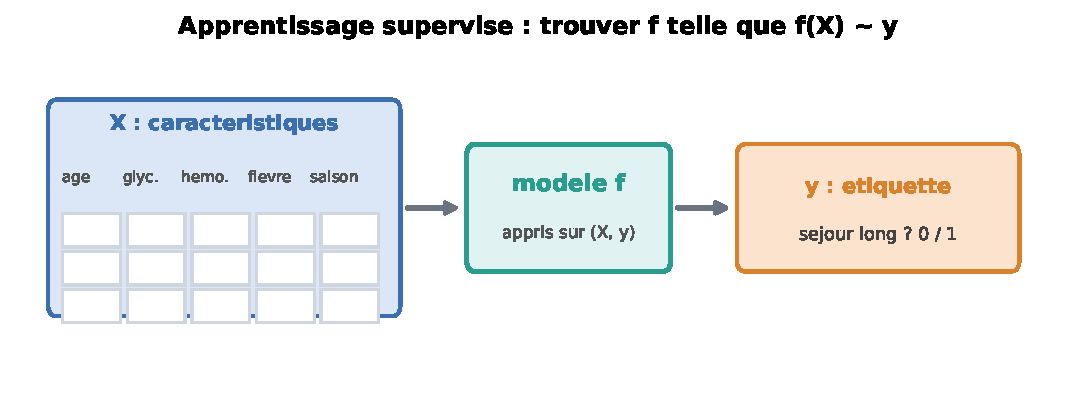
\includegraphics[width=0.58\linewidth]{f_supervised}
\vspace{-2pt}

{\scriptsize Le registre contient $10\,000$ patients pour lesquels la réponse est \emph{connue}. L'objectif est d'en extraire une règle de prédiction applicable aux patients futurs.}
\end{frame}

\begin{frame}{L'apprentissage supervisé, formellement}
\begin{ucaddef}[Définition]
{\small L'\textbf{apprentissage supervisé} consiste à construire, à partir d'exemples étiquetés $(x_i, y_i)$, une fonction de prédiction qui associe à toute entrée une sortie.}
\end{ucaddef}
\ucadformula{f : \mathcal{X} \longrightarrow \mathcal{Y}, \qquad f(x) \approx y}
{\small $\mathcal{X}$ est l'espace des entrées (ici, les mesures d'un patient) et $\mathcal{Y}$ l'espace des sorties (ici, $\{0,1\}$ : séjour court ou long). Le modèle \emph{est} la fonction $f$ ; l'apprentissage consiste à la choisir à partir des données.}
\end{frame}

\begin{frame}{Les données : la matrice de design $X$}
\begin{ucaddef}[Organisation des données]
{\small Les $n$ exemples s'empilent dans une matrice $X \in \mathbb{R}^{n\times d}$ — une \textbf{ligne} par exemple, une \textbf{colonne} par caractéristique — et leurs réponses dans le vecteur $y$. Le couple $(X,y)$ est le jeu d'apprentissage.}
\end{ucaddef}
\begin{ucadex}[Premières lignes réelles de DataSANTÉ-221]
{\footnotesize \begin{tabular}{c|ccccc|c}
 & âge & glycémie & hémoglobine & fièvre & saison & séjour long\\\hline
$x_1$ & $47$ & $9{,}3$ & $11{,}8$ & $38{,}0$ & $0$ & $y_1 = 0$\\
$x_2$ & $18$ & $5{,}1$ & $13{,}0$ & $39{,}5$ & $1$ & $y_2 = 0$\\
$x_3$ & $56$ & $7{,}2$ & $9{,}5$ & $37{,}1$ & $1$ & $y_3 = 1$\\
\end{tabular}}
\end{ucadex}

\end{frame}

% Slide coupée en deux : le tableau et la notation matricielle ne tenaient pas ensemble dans le
% cadre de 700 unités (941 px mesurés). Rien n'est retiré.
\begin{frame}{Les mêmes données, en notation matricielle}
\begin{ucadex}[$X$ et $y$ de DataSANTÉ-221]
{\footnotesize \[ X=\begin{pmatrix} 47 & 9{,}3 & 11{,}8 & 38{,}0 & 0\\ 18 & 5{,}1 & 13{,}0 & 39{,}5 & 1\\ 56 & 7{,}2 & 9{,}5 & 37{,}1 & 1\\ \vdots & \vdots & \vdots & \vdots & \vdots \end{pmatrix} \in \mathbb{R}^{10000\times 5} \qquad y=\begin{pmatrix} 0\\ 0\\ 1\\ \vdots \end{pmatrix} \in \{0,1\}^{10000} \]}
\end{ucadex}

\end{frame}

% #####################################################################
\section{Entraîner et évaluer}

\begin{frame}[fragile]{Le protocole scikit-learn : fit, predict, score}
\begin{lstlisting}
from sklearn.tree import DecisionTreeClassifier

modele = DecisionTreeClassifier(max_depth=4, random_state=0)
modele.fit(X_train, y_train)        # apprendre f a partir des exemples
y_pred = modele.predict(X_test)     # appliquer f a de nouveaux patients
modele.score(X_test, y_test)        # mesurer la qualite des predictions
\end{lstlisting}
{\small Ce triptyque \texttt{fit} / \texttt{predict} / \texttt{score} est identique pour tous les modèles de \texttt{scikit-learn} ; seule la classe instanciée change.}
\end{frame}

\begin{frame}{Mesurer la qualité : perte et risque empirique}
\begin{ucaddef}[La perte 0/1]
{\small Pour une prédiction donnée, la \textbf{perte} vaut $0$ si elle est correcte, $1$ sinon. Le \textbf{risque empirique} est la moyenne des pertes sur un jeu de données.}
\end{ucaddef}
\ucadformula{\widehat{R}(f) = \frac{1}{n}\sum_{i=1}^{n} \mathbf{1}\big[f(x_i) \neq y_i\big] \qquad \text{accuracy} = 1 - \widehat{R}(f)}
{\small La somme compte les erreurs ; la division par $n$ en donne la proportion. L'accuracy est la proportion complémentaire : celle des prédictions correctes.}
\end{frame}

\begin{frame}{Exemple — comparer $y$ et $\hat y$}
\begin{ucadex}[Exemple numérique]
{\small Cinq patients du test : comparaison composante par composante du vecteur des réponses $y$ et du vecteur des prédictions $\hat y = f(X_{\text{test}})$.
\begin{center}\begin{tabular}{l|ccccc}
patient & $1$ & $2$ & $3$ & $4$ & $5$\\\hline
réponse $y_i$ & $1$ & $0$ & $1$ & $1$ & $0$\\
prédiction $\hat y_i$ & $1$ & $0$ & $0$ & $1$ & $1$\\
correcte ? & oui & oui & \textbf{non} & oui & \textbf{non}\\
\end{tabular}\end{center}
Trois prédictions correctes sur cinq : accuracy $= \dfrac{3}{5} = \mathbf{0{,}60}$ ; risque $= \dfrac{2}{5} = \mathbf{0{,}40}$.}
\end{ucadex}
{\small La mesure repose toujours sur cette comparaison des deux vecteurs — c'est elle que \texttt{score} automatise.}
\end{frame}

\begin{frame}{Exercice — calcul d'une accuracy}
\begin{ucadrec}[Énoncé]
{\small Sur $60$ patients du jeu de test, le modèle commet $15$ erreurs. Calculer l'accuracy et le risque empirique.}
\end{ucadrec}
\pause
\begin{ucadex}[Correction]
{\small Prédictions correctes $= 60-15 = 45$, d'où accuracy $= \dfrac{45}{60} = \mathbf{0{,}75}$ et risque $= \dfrac{15}{60} = \mathbf{0{,}25}$. Les deux quantités sont complémentaires : $\text{accuracy} = 1 - \widehat{R}$.}
\end{ucadex}
\end{frame}

\begin{frame}{Le protocole train/test}
\begin{ucaddef}[Pourquoi séparer les données]
{\small La performance qui importe est celle sur des patients \textbf{jamais vus} : la \textbf{généralisation}. On réserve donc une fraction des données (le \textbf{test}, ici $20\,\%$), exclue de l'apprentissage, pour estimer cette performance honnêtement.}
\end{ucaddef}
\centering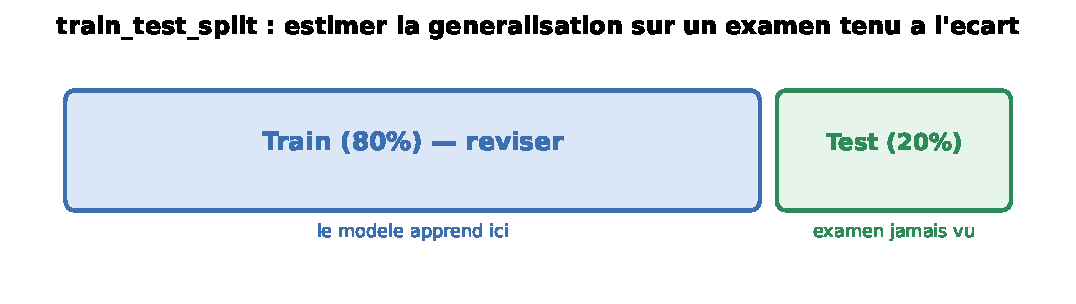
\includegraphics[width=0.82\linewidth]{f_traintest}
\vspace{-2pt}

{\scriptsize Découpage \emph{aléatoire} et \emph{stratifié} : $8000$ patients pour apprendre, $2000$ pour évaluer. Un score mesuré sur le jeu d'entraînement lui-même serait systématiquement optimiste.}
\end{frame}

\begin{frame}{Exercice — dimensions et découpage}
\begin{ucadrec}[Énoncé]
{\small DataSANTÉ-221 : $n=10\,000$ patients, $d=5$ caractéristiques. \textbf{(a)} Quelle est la taille de la matrice $X$ ? \textbf{(b)} Si l'on choisissait plutôt \texttt{test\_size=0.25}, combien de patients iraient dans le jeu d'entraînement et dans le jeu de test ?}
\end{ucadrec}
\pause
\begin{ucadex}[Correction]
{\small \textbf{(a)} $X \in \mathbb{R}^{10000\times 5}$ : une ligne par patient, une colonne par caractéristique. \textbf{(b)} Test $=25\,\%$ de $10\,000 = \mathbf{2500}$ ; entraînement $= \mathbf{7500}$.}
\end{ucadex}
\end{frame}

\begin{frame}{La référence minimale : la baseline}
\begin{ucaddef}[Définition]
{\small La \textbf{baseline} est le prédicteur trivial qui répond toujours la classe majoritaire. Tout modèle digne d'intérêt doit la dépasser ; un score ne s'interprète que \emph{relativement} à elle.}
\end{ucaddef}
\begin{ucadex}[Exemple numérique]
{\small Sur DataSANTÉ-221, les classes sont quasi équilibrées ($5045$ contre $4955$) : la baseline atteint $\mathbf{0{,}5045}$. L'arbre de profondeur $4$ obtient $0{,}7655$ sur le test — soit $26$ points au-dessus de la baseline : le modèle a réellement appris.}
\end{ucadex}
\end{frame}

% #####################################################################
\section{L'arbre de décision}

\begin{frame}{Le principe : une suite de questions}
\begin{ucadfront}[Analogie]
{\small Aux urgences, le médecin de tri ne résout pas d'équation : il pose une question, puis une autre — « la glycémie dépasse-t-elle $7$ ? », « plus de $60$ ans ? » — et chaque réponse rétrécit le champ des possibles, jusqu'au pronostic. L'arbre de décision reproduit ce geste, à une différence près : l'ordre des questions et la valeur des seuils ne viennent pas de l'expérience du praticien — ils sont \emph{calculés à partir des données}.}
\end{ucadfront}
\centering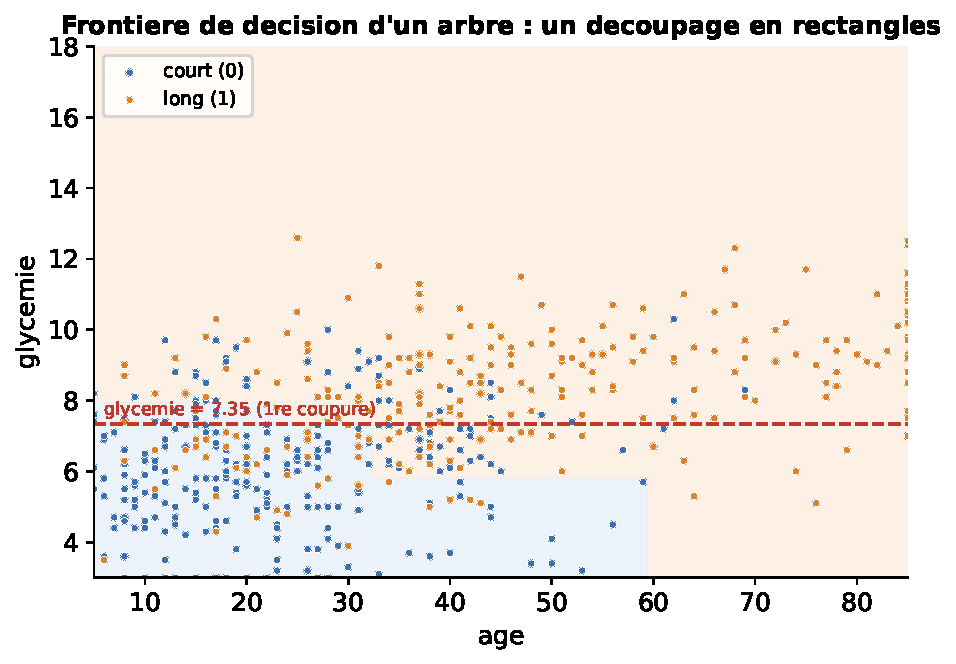
\includegraphics[width=0.27\linewidth]{f_boundary}
\vspace{-2pt}

{\scriptsize Chaque question trace une frontière verticale ou horizontale : l'arbre découpe le plan en \textbf{rectangles} de décision.}
\end{frame}

\begin{frame}{L'arbre, formellement}
\begin{ucaddef}[Modèle]
{\small Un arbre partitionne l'espace des entrées en $M$ régions disjointes $R_1, \dots, R_M$ (les feuilles) et prédit une valeur constante dans chacune.}
\end{ucaddef}
\ucadformula{f(x) = \sum_{m=1}^{M} \hat c_m \, \mathbf{1}\big[x \in R_m\big]}
{\small L'indicatrice $\mathbf{1}[\cdot]$ sélectionne la région contenant $x$ ; $\hat c_m$ est la classe majoritaire des exemples d'entraînement tombés dans $R_m$. Chaque nœud interne applique une \textbf{coupure} $(j, s)$ : « la caractéristique $j$ dépasse-t-elle le seuil $s$ ? »}
\end{frame}

\begin{frame}{Exemple — évaluer $f(x)$ terme à terme}
\begin{ucadex}[Un arbre à trois régions]
{\small Un petit arbre découpe le plan (glycémie, âge) en $M=3$ régions, avec leurs classes majoritaires :
\begin{center}\small
$R_1 = \{\text{glycémie} \le 7\}$, $\hat c_1 = 0$ ; \quad
$R_2 = \{\text{glycémie} > 7,\ \text{âge} \le 50\}$, $\hat c_2 = 0$ ; \quad
$R_3 = \{\text{glycémie} > 7,\ \text{âge} > 50\}$, $\hat c_3 = 1$.
\end{center}
Patient $x = (\text{glycémie } 9{,}0,\ \text{âge } 62)$ : il n'appartient qu'à $R_3$, donc $\mathbf{1}[x \in R_1] = 0$, $\mathbf{1}[x \in R_2] = 0$, $\mathbf{1}[x \in R_3] = 1$.
\[ f(x) = \hat c_1 \times 0 + \hat c_2 \times 0 + \hat c_3 \times 1 = 0 + 0 + 1 = \mathbf{1} \quad \text{(séjour long).} \]}
\end{ucadex}
{\small Les régions étant disjointes, une seule indicatrice vaut $1$ : la somme \emph{sélectionne} la prédiction de la région où tombe $x$. Autre patient, $x' = (5{,}2,\ 70)$ : indicatrices $(1, 0, 0)$, d'où $f(x') = \hat c_1 = \mathbf{0}$.}
\end{frame}

\begin{frame}{La pureté d'un nœud : l'idée}
\begin{ucaddef}[Les chiffres d'abord]
{\small Un groupe est \textbf{pur} lorsqu'il ne contient qu'une seule classe. L'\textbf{impureté} mesure son désordre : $0$ pour un groupe pur, $0{,}88$ bit pour un mélange $70/30$, $1$ bit pour un mélange $50/50$ — le désordre maximal.}
\end{ucaddef}
\centering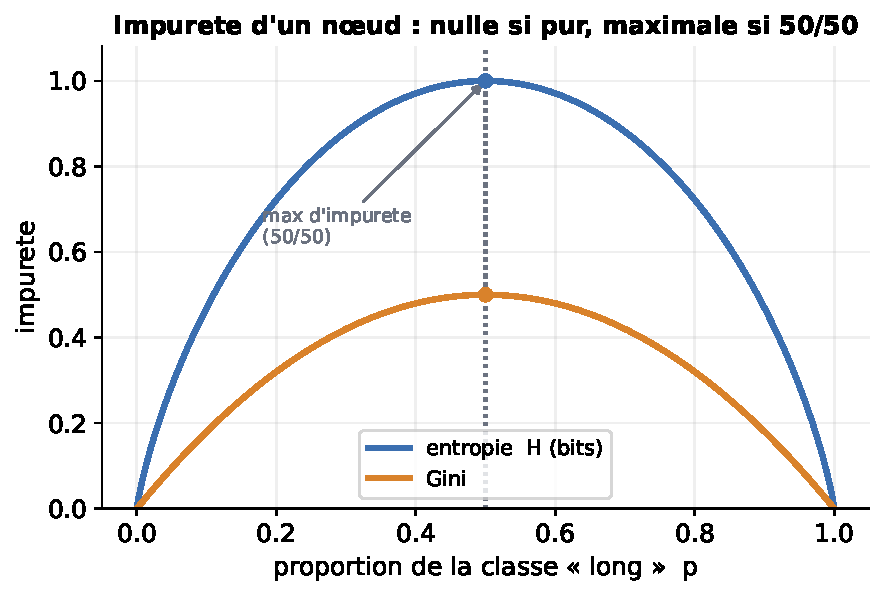
\includegraphics[width=0.38\linewidth]{f_impurity}
\vspace{-3pt}

{\scriptsize L'\textbf{entropie} $H$ et l'\textbf{indice de Gini} $G$ selon la proportion $p$ : nulles aux extrêmes (pureté), maximales à $p=0{,}5$.}
\end{frame}

\begin{frame}{L'entropie, formellement}
\begin{ucaddef}[L'idée en une phrase]
{\small L'entropie mesure le \textbf{désordre} d'un nœud — la surprise moyenne de son contenu : nulle quand l'issue est jouée d'avance (nœud pur), maximale quand les deux classes sont à égalité.}
\end{ucaddef}
\ucadformula{H(p) \;=\; -\,p\,\log_2 p \;-\; (1-p)\,\log_2(1-p)}
{\small $p$ est la proportion d'une classe dans le nœud ; l'unité est le \textbf{bit}. Rappel : $\log_2 x$ est l'exposant à donner à $2$ pour obtenir $x$ ($\log_2 4 = 2$, $\log_2 0{,}25 = -2$) — négatif pour $0<x<1$, d'où les signes moins.}
\begin{ucadex}[Exemple numérique]
{\small Nœud à $25\,\%$ de séjours longs ($p=0{,}25$) :
$H = -0{,}25\log_2 0{,}25 - 0{,}75\log_2 0{,}75 = 0{,}25\times 2 + 0{,}75\times 0{,}415 = 0{,}5 + 0{,}311 = \mathbf{0{,}811}$ bit.}
\end{ucadex}
\end{frame}

\begin{frame}{Exercice — calcul d'une entropie}
\begin{ucadrec}[Énoncé]
{\small Un nœud contient $90\,\%$ de séjours longs ($p = 0{,}9$). Calculer son entropie, sachant que $\log_2 0{,}9 = -0{,}152$ et $\log_2 0{,}1 = -3{,}322$. Commenter le résultat.}
\end{ucadrec}
\pause
\begin{ucadex}[Correction]
{\small $H = -0{,}9\times(-0{,}152) - 0{,}1\times(-3{,}322) = 0{,}137 + 0{,}332 = \mathbf{0{,}469}$ bit. Le nœud est déjà bien ordonné ($90/10$) : son impureté est moins de la moitié du maximum — il reste peu de désordre à réduire.}
\end{ucadex}
\end{frame}

\begin{frame}{L'indice de Gini}
\begin{ucaddef}[L'idée en une phrase]
{\small L'indice de Gini mesure le même désordre par une question simple : si l'on classait un patient \textbf{au hasard}, selon les proportions du nœud, quelle serait la probabilité de se tromper ?}
\end{ucaddef}
\ucadformula{G(p) \;=\; 1 - p^2 - (1-p)^2 \;=\; 2\,p\,(1-p)}
{\small Maximum $0{,}5$ lorsque les classes sont à égalité ($p=0{,}5$) ; nul si le nœud est pur — il est alors impossible de se tromper.}
\begin{ucadex}[Exemple numérique]
{\small $G(0{,}5) = 2\times 0{,}5\times 0{,}5 = \mathbf{0{,}5}$ ; \quad $G(0{,}25) = 2\times 0{,}25\times 0{,}75 = \mathbf{0{,}375}$ ; \quad $G(1) = \mathbf{0}$.}
\end{ucadex}
{\small Entropie et Gini classent les coupures presque toujours dans le \emph{même ordre} ; Gini, sans logarithme, est moins coûteux — c'est le critère par défaut de \texttt{scikit-learn}. La suite utilise l'entropie, plus interprétable (en bits).}
\end{frame}

\begin{frame}{La coupure et le gain d'information}
\begin{ucaddef}[Le principe de sélection]
{\small Une \textbf{coupure} $(j,s)$ scinde un nœud selon « la caractéristique $j$ dépasse-t-elle le seuil $s$ ? ». Une bonne coupure produit des enfants \emph{plus purs} que le parent : le \textbf{gain} mesure cette baisse d'impureté.}
\end{ucaddef}
\ucadformula{\text{Gain}(j,s) \;=\; H_{\text{parent}} \;-\; \big(\pi_g\, H_g + \pi_d\, H_d\big) \qquad (j^\star, s^\star) = \arg\max_{(j,s)}\, \text{Gain}(j,s)}
{\small $\pi_g$ et $\pi_d$ sont les proportions d'exemples envoyées à gauche et à droite : l'impureté des enfants est une \emph{moyenne pondérée}. L'algorithme évalue \textbf{toutes} les coupures possibles et retient celle du gain maximal — puis recommence dans chaque enfant, récursivement.}
\end{frame}

% ---------- construction de bout en bout ----------
\begin{frame}{Construire un arbre à la main — les huit patients}
\begin{ucaddef}[Un exemple de bout en bout]
{\small Pour observer l'algorithme à l'œuvre, on construit \emph{intégralement} un arbre sur huit patients et deux caractéristiques — une \textbf{ligne} par patient, comme dans la matrice $X$.}
\end{ucaddef}
\begin{ucadex}[Les huit patients]
{\scriptsize \renewcommand{\arraystretch}{0.92}\begin{tabular}{c|cc|c}
patient & glycémie & fièvre & séjour long\\\hline
$x_1$ & $5{,}0$ & $37{,}3$ & $y_1 = 1$\\
$x_2$ & $6{,}0$ & $37{,}0$ & $y_2 = 0$\\
$x_3$ & $6{,}5$ & $37{,}6$ & $y_3 = 0$\\
$x_4$ & $7{,}0$ & $38{,}2$ & $y_4 = 0$\\
$x_5$ & $8{,}0$ & $37{,}9$ & $y_5 = 1$\\
$x_6$ & $9{,}0$ & $38{,}5$ & $y_6 = 1$\\
$x_7$ & $10{,}0$ & $39{,}1$ & $y_7 = 1$\\
$x_8$ & $12{,}0$ & $38{,}8$ & $y_8 = 0$\\
\end{tabular}}
\end{ucadex}
\end{frame}

\begin{frame}{La racine : quatre longs, quatre courts}
{\small Quatre séjours longs, quatre courts : la racine est au désordre maximal, $H_{\text{racine}} = \mathbf{1{,}000}$ bit ($G = 0{,}5$).}
\end{frame}

\begin{frame}{Étape 1 — le duel des coupures candidates}
\begin{ucadex}[Trois candidates évaluées]
{\footnotesize
\textbf{A. glycémie $\le 7$} : gauche $=\{1,0,0,0\}$, droite $=\{1,1,1,0\}$ $\to$ gain $= \mathbf{0{,}189}$ bit (détail page suivante).\\[2pt]
\textbf{B. fièvre $\le 38$} : gauche $=\{1,0,0,1\}$ ($p=0{,}5$, $H=1$), droite $=\{0,1,1,0\}$ ($p=0{,}5$, $H=1$) $\to$ gain $= 1 - \tfrac{4}{8}\cdot 1 - \tfrac{4}{8}\cdot 1 = \mathbf{0}$ bit.\\[2pt]
\textbf{C. glycémie $\le 9{,}5$} : gauche $=\{1,0,0,0,1,1\}$ ($p=0{,}5$, $H=1$), droite $=\{1,0\}$ ($p=0{,}5$, $H=1$) $\to$ gain $= \mathbf{0}$ bit.}
\end{ucadex}
{\small La coupure B scinde sans trier : ses enfants restent au désordre maximal — un gain \emph{nul} malgré la séparation. L'argmax (sur \emph{toutes} les coupures des deux caractéristiques) retient \textbf{A : glycémie $\le 7$}.}
\end{frame}

\begin{frame}{Étape 1 — le calcul détaillé du gain retenu}
\begin{ucadex}[Coupure glycémie $\le 7$ pas à pas]
{\small Gauche (patients $1$–$4$) : étiquettes $\{1,0,0,0\}$, $p_g = \tfrac{1}{4} = 0{,}25$, $H_g = \mathbf{0{,}811}$ (calculé plus haut).\\
Droite (patients $5$–$8$) : étiquettes $\{1,1,1,0\}$, $p_d = 0{,}75$, $H_d = \mathbf{0{,}811}$ (symétrie de $H$).\\[4pt]
$\text{Gain} = 1{,}000 - \Big(\dfrac{4}{8}\times 0{,}811 + \dfrac{4}{8}\times 0{,}811\Big) = 1{,}000 - 0{,}811 = \mathbf{0{,}189}$ bit.}
\end{ucadex}
{\small Le même calcul avec Gini : $0{,}5 - 0{,}375 = \mathbf{0{,}125}$ — un autre chiffre, le \emph{même} verdict. Les deux enfants restent impurs ($0{,}811$ bit) : la récursion continue.}
\end{frame}

\begin{frame}{Étape 2 — purifier le nœud gauche}
\begin{ucadex}[Nœud gauche : glycémies 5 ; 6 ; 6{,}5 ; 7 — étiquettes 1 ; 0 ; 0 ; 0]
{\small Coupure \textbf{glycémie $\le 5{,}5$} : gauche $=\{1\}$ (pur, $H=0$), droite $=\{0,0,0\}$ (pur, $H=0$).\\[4pt]
$\text{Gain} = 0{,}811 - \Big(\dfrac{1}{4}\times 0 + \dfrac{3}{4}\times 0\Big) = \mathbf{0{,}811}$ bit — tout le désordre restant est absorbé.}
\end{ucadex}
{\small Les deux enfants sont \textbf{purs} : ce sont des \textbf{feuilles}. La branche gauche est terminée — aucune coupure supplémentaire n'apporterait de gain.}
\end{frame}

\begin{frame}{Étape 2 — purifier le nœud droit}
\begin{ucadex}[Nœud droit : glycémies 8 ; 9 ; 10 ; 12 — étiquettes 1 ; 1 ; 1 ; 0]
{\small Coupure \textbf{glycémie $\le 11$} : gauche $=\{1,1,1\}$ (pur), droite $=\{0\}$ (pur).\\[4pt]
$\text{Gain} = 0{,}811 - 0 = \mathbf{0{,}811}$ bit. Deux feuilles pures : la branche droite est terminée.}
\end{ucadex}
{\small L'algorithme s'arrête : toutes les feuilles sont pures. L'arbre complet a été obtenu par trois applications du \emph{même} principe — l'argmax du gain, appliqué récursivement.}
\end{frame}

\begin{frame}{L'arbre final, et sa vérification}
\centering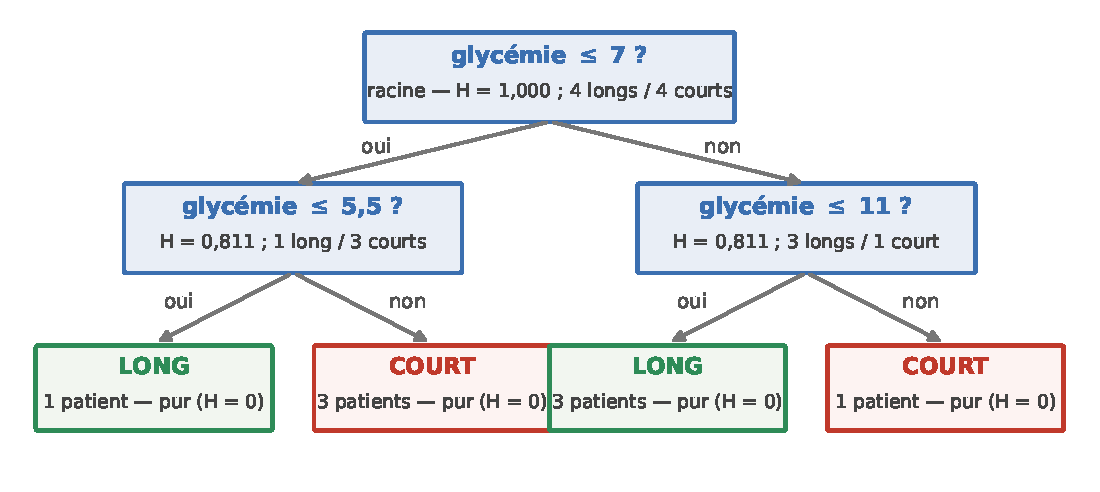
\includegraphics[width=0.72\linewidth]{f_minitree}
\vspace{-2pt}

{\scriptsize \texttt{DecisionTreeClassifier(criterion="entropy")} entraîné sur ces huit patients reproduit \textbf{exactement} cet arbre (seuils aux points médians : $7{,}5$ ; $5{,}5$ ; $11$) — score $8/8$. Feuilles pures sur huit patients : l'arbre a \emph{mémorisé} l'échantillon ; ce constat annonce la question du sur-apprentissage, traitée plus loin.}
\end{frame}

\begin{frame}{Exercice — un gain à la main}
\begin{ucadrec}[Énoncé]
{\small Sur le nœud droit (étiquettes $\{1,1,1,0\}$, $H = 0{,}811$), calculer le gain de la coupure \textbf{glycémie $\le 9{,}5$} (gauche $=\{1,1\}$, droite $=\{1,0\}$) et le comparer au gain de la coupure retenue ($0{,}811$).}
\end{ucadrec}
\pause
\begin{ucadex}[Correction]
{\small $H_g = H(1) = 0$ (pur) ; $H_d = H(0{,}5) = 1$.
$\text{Gain} = 0{,}811 - \Big(\dfrac{2}{4}\times 0 + \dfrac{2}{4}\times 1\Big) = 0{,}811 - 0{,}5 = \mathbf{0{,}311}$ bit — inférieur à $0{,}811$ : l'argmax écarte cette candidate, qui laisse un enfant au désordre maximal.}
\end{ucadex}
\end{frame}

\begin{frame}{La première coupure réelle}
\begin{ucadex}[Exemple numérique]
{\small Sur les $8000$ patients d'entraînement, la coupure optimale trouvée par l'algorithme est \textbf{glycémie $\le 7{,}35$}, avec un gain de $\mathbf{0{,}155}$ bit — la meilleure parmi toutes les coupures possibles sur les cinq caractéristiques.}
\end{ucadex}
\centering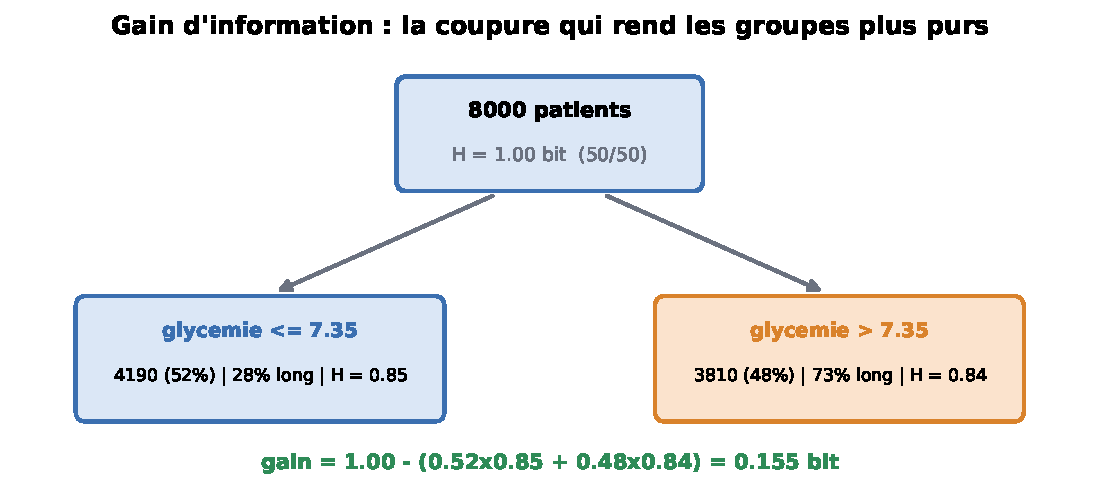
\includegraphics[width=0.48\linewidth]{f_infogain}
\vspace{-2pt}

{\scriptsize À gauche de la coupure, les séjours courts dominent ; à droite, les séjours longs. Même principe que sur les huit patients — appliqué à $8000$. Au TP : ce gain de $0{,}155$ bit est recalculé à la main, ainsi que la construction complète de l'arbre jouet.}
\end{frame}

\begin{frame}{Lire une prédiction : du chemin à la feuille}
\centering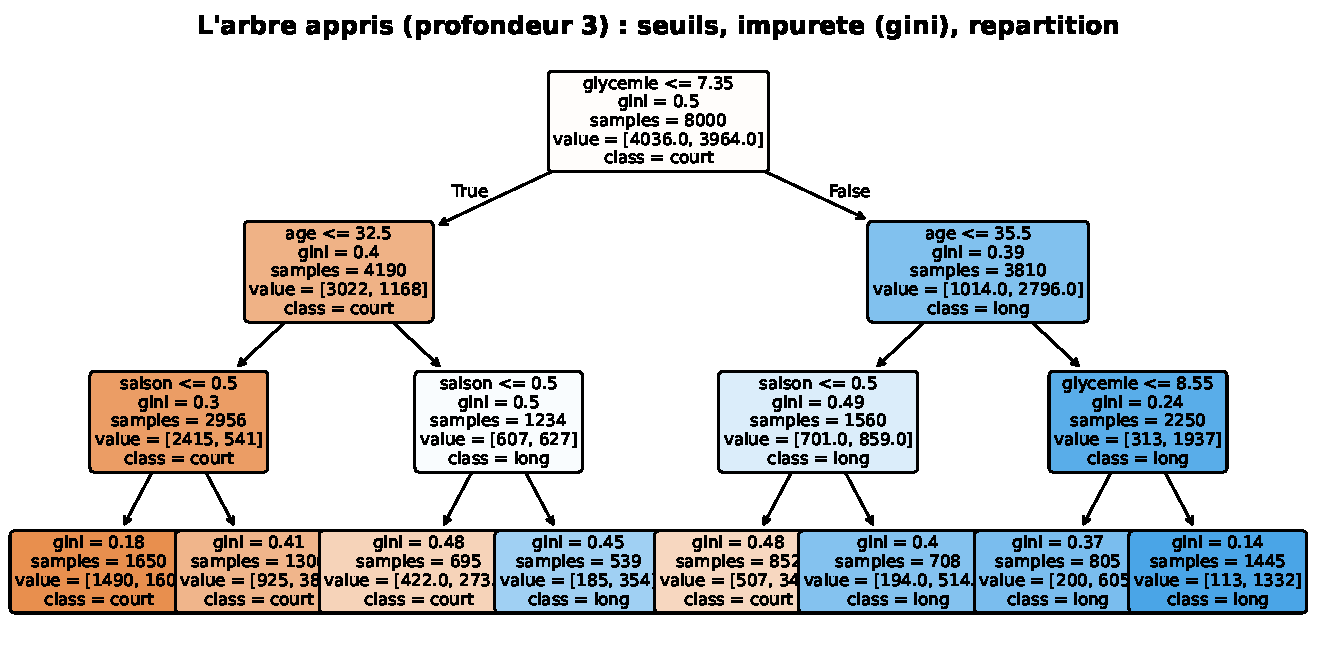
\includegraphics[width=0.80\linewidth]{f_tree}
\vspace{-2pt}

{\scriptsize Pour prédire, on suit le chemin des réponses de la racine jusqu'à une feuille. Exemple : un patient de $60$ ans, glycémie $9{,}0$ — la branche droite conduit à une feuille à $95\,\%$ « long », d'où $f(x) = 1$ avec une confiance de $0{,}95$.}
\end{frame}

\begin{frame}{Exercice — suivre un chemin}
\begin{ucadrec}[Énoncé]
{\small Arbre simplifié : racine « glycémie $\le 7{,}35$ ? » — \textbf{oui} $\to$ feuille à $88\,\%$ « court » ; \textbf{non} $\to$ « âge $\le 50$ ? » — \textbf{oui} $\to$ feuille à $60\,\%$ « long », \textbf{non} $\to$ feuille à $95\,\%$ « long ». Déterminer la prédiction et la confiance pour un patient de $45$ ans dont la glycémie vaut $8{,}2$.}
\end{ucadrec}
\pause
\begin{ucadex}[Correction]
{\small $8{,}2 > 7{,}35 \to$ branche droite ; $45 \le 50 \to$ feuille « long » à $60\,\%$. Prédiction $f(x) = \mathbf{1}$, confiance $\mathbf{0{,}60}$ — une prédiction peu assurée : la feuille est presque partagée.}
\end{ucadex}
\end{frame}

% #####################################################################
\section{Sous-apprentissage et sur-apprentissage}

\begin{frame}{La profondeur contrôle la complexité}
\begin{ucaddef}[Un réglage central]
{\small La profondeur maximale (\texttt{max\_depth}) borne le nombre de questions successives. Elle détermine la \textbf{complexité} du modèle — et son comportement face aux données.}
\end{ucaddef}
\begin{ucadex}[Exemple numérique]
{\small \begin{tabular}{l|cc}
 & score train & score test\\\hline
profondeur $4$ & $0{,}7738$ & $\mathbf{0{,}7655}$\\
profondeur illimitée & $0{,}9999$ & $0{,}6995$\\
\end{tabular}}
\end{ucadex}
{\small L'arbre illimité mémorise presque parfaitement le jeu d'entraînement — et prédit \emph{moins bien} les patients nouveaux. Mémoriser n'est pas généraliser.}
\end{frame}

\begin{frame}{La courbe de complexité}
\centering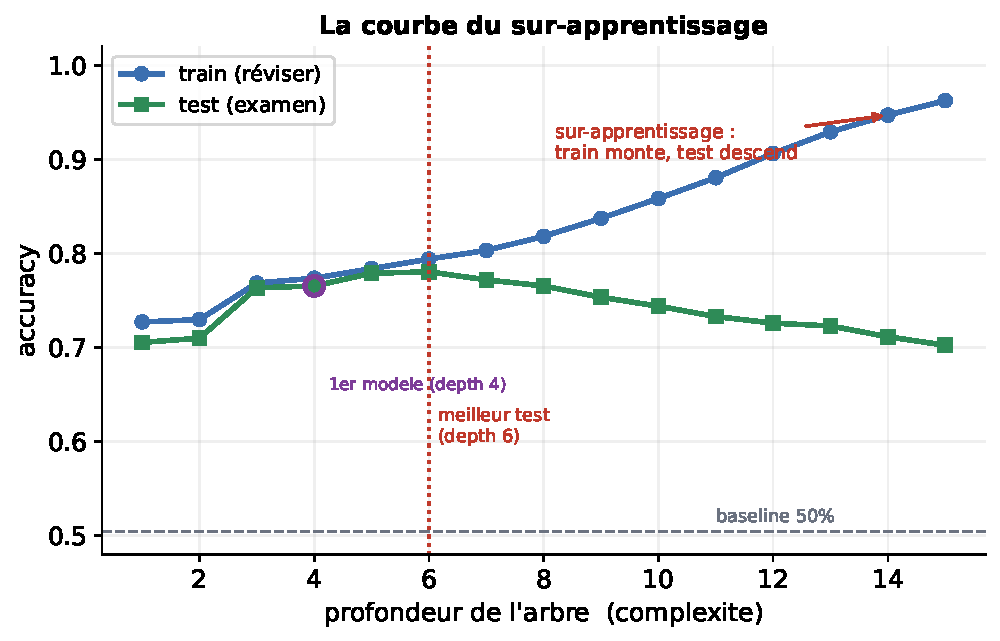
\includegraphics[width=0.58\linewidth]{f_overfit}
\vspace{-2pt}

{\scriptsize Le score d'entraînement croît avec la profondeur ; le score de test culmine puis \textbf{redescend}. À gauche du sommet, le modèle est trop simple (\textbf{sous-apprentissage}) ; à droite, il apprend les particularités du jeu d'entraînement, bruit compris (\textbf{sur-apprentissage}).}
\end{frame}

\begin{frame}{Exercice — diagnostiquer un modèle}
\begin{ucadrec}[Énoncé]
{\small Trois modèles, trois couples (score train, score test) : \textbf{A} $(0{,}71;\ 0{,}70)$ ; \textbf{B} $(0{,}78;\ 0{,}76)$ ; \textbf{C} $(0{,}99;\ 0{,}68)$. Diagnostiquer chacun.}
\end{ucadrec}
\pause
\begin{ucadex}[Correction]
{\small \textbf{A} : scores faibles et proches — \textbf{sous-apprentissage} (modèle trop simple). \textbf{B} : scores corrects et proches — bon compromis. \textbf{C} : écart majeur entre train et test — \textbf{sur-apprentissage} caractérisé. Le diagnostic repose toujours sur la \emph{paire} de scores, jamais sur un seul.}
\end{ucadex}
\end{frame}

% #####################################################################
\section{Le compromis biais-variance}

\begin{frame}{Deux sources d'erreur}
\begin{ucadfront}[Analogie]
{\small Un tailleur doit livrer un boubou à un client, après plusieurs essayages. Premier excès : il coud sur un \textbf{patron unique}, taille moyenne, sans toucher aux mesures — quel que soit l'essayage, la manche est trop courte des \emph{mêmes} trois centimètres. L'erreur est systématique et se répète à l'identique : c'est le \textbf{biais}, l'excès de rigidité. Second excès, sur le \emph{même} boubou : à chaque essayage, il reprend toute la coupe pour épouser les mesures du jour — y compris le pull épais que le client portait ce jour-là. Chaque version diffère de la précédente : c'est la \textbf{variance}, l'excès de sensibilité aux données du jour.}
\end{ucadfront}
{\small Le sous-apprentissage est un excès de biais ; le sur-apprentissage, un excès de variance. Toute la pratique du ML consiste à doser entre les deux.}
\end{frame}

\begin{frame}{La cible : visualiser biais et variance}
\centering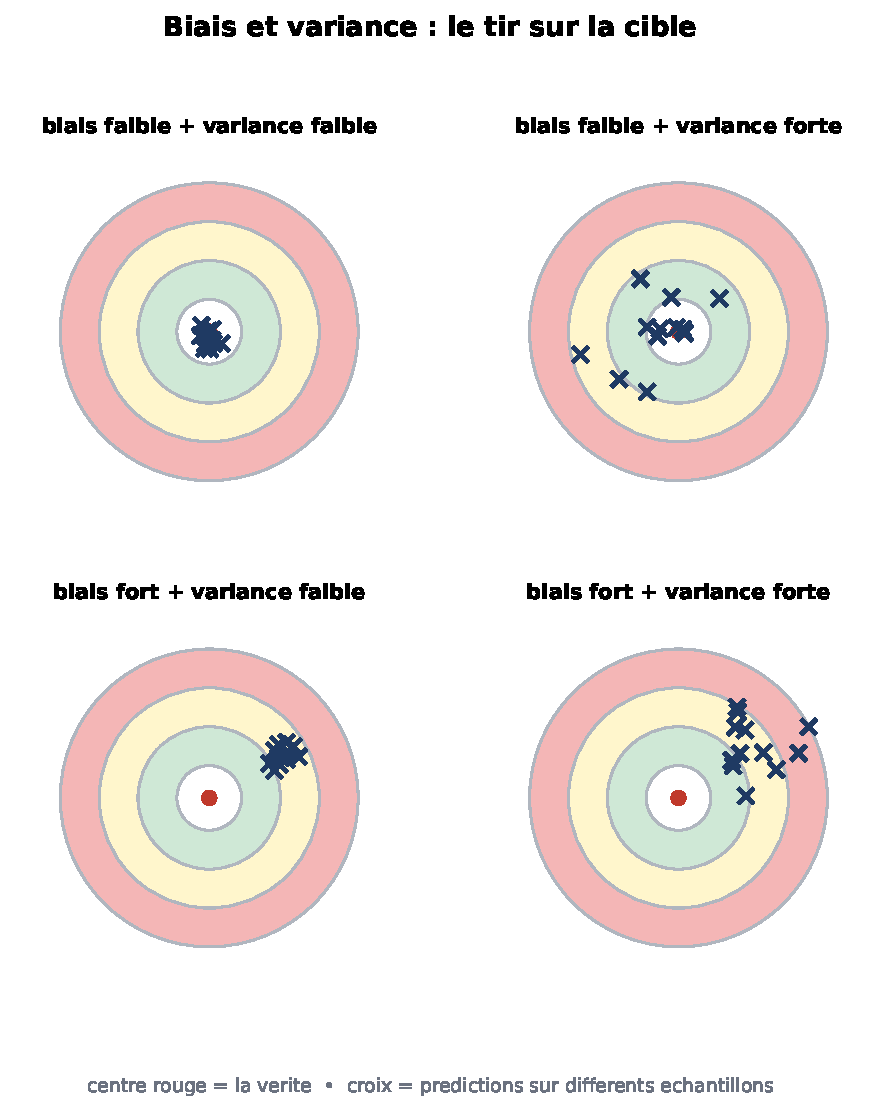
\includegraphics[width=0.26\linewidth]{f_dartboard}
\vspace{-3pt}

{\scriptsize Chaque impact est un modèle entraîné sur un échantillon différent. \textbf{Biais} : impacts décalés du centre, systématiquement — le boubou au patron unique, toujours faux de la même manière. \textbf{Variance} : impacts dispersés — le boubou recousu à chaque essayage, différent à chaque fois. Le cas favorable — groupés au centre — exige de réduire les deux.}
\end{frame}

\begin{frame}{Trois ajustements, une même donnée}
\centering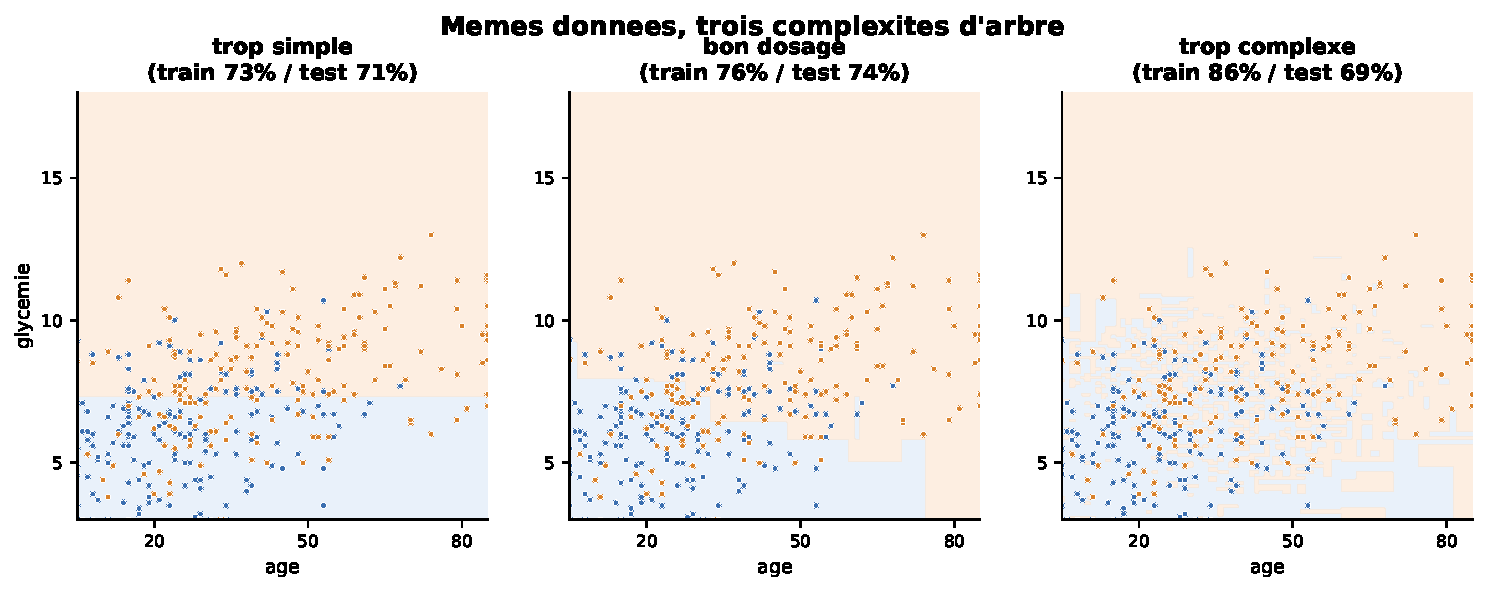
\includegraphics[width=0.99\linewidth]{f_threefits}
\vspace{-2pt}

{\scriptsize Profondeur $1$ : frontière trop grossière, biais dominant (test $0{,}71$). Profondeur $4$ : compromis (test $0{,}77$). Profondeur illimitée : frontière déchiquetée épousant chaque point, variance dominante (test $0{,}70$).}
\end{frame}

\begin{frame}{La décomposition de l'erreur}
\ucadformula{\mathbb{E}\big[\text{erreur}\big] = \underbrace{\text{biais}^2}_{\text{rigidité}} + \underbrace{\text{variance}}_{\text{instabilité}} + \underbrace{\sigma^2}_{\text{bruit irréductible}}}
{\small L'erreur attendue d'un modèle se décompose en trois termes : l'erreur systématique (biais), la sensibilité à l'échantillon (variance), et le bruit propre aux données, qu'aucun modèle ne peut éliminer. Augmenter la complexité réduit le biais mais accroît la variance — d'où l'existence d'un optimum intermédiaire.}
\begin{ucadpiege}[Erreur fréquente]
{\small Viser un score d'entraînement parfait. Le terme de bruit $\sigma^2$ rend cet objectif illusoire : un score train de $100\,\%$ signale presque toujours que la variance a explosé.}
\end{ucadpiege}
\end{frame}

% #####################################################################
\section{Interpréter le modèle}

\begin{frame}{L'importance des caractéristiques}
\begin{ucaddef}[Définition]
{\small L'\textbf{importance} d'une caractéristique est la part du gain total d'impureté apportée par les coupures qui l'utilisent. Les importances sont normalisées : leur somme vaut $1$.}
\end{ucaddef}
\centering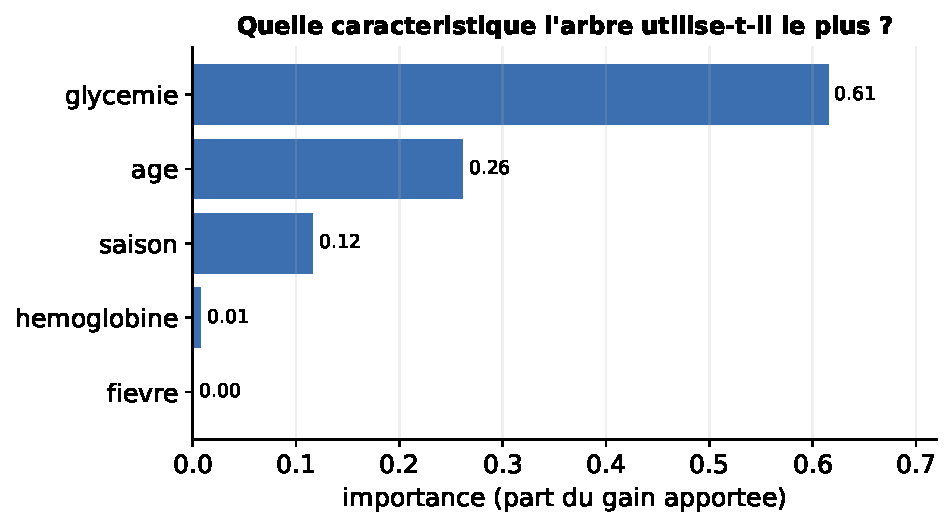
\includegraphics[width=0.50\linewidth]{f_importance}
\vspace{-2pt}

{\scriptsize Sur DataSANTÉ-221 : glycémie $0{,}615$, âge $0{,}261$, saison $0{,}116$, hémoglobine $0{,}008$, fièvre $0{,}000$. La glycémie domine ; la fièvre n'est utilisée par aucune coupure.}
\end{frame}

\begin{frame}{Exercice — lire des importances}
\begin{ucadrec}[Énoncé]
{\small Importances de l'arbre : glycémie $0{,}615$, âge $0{,}261$, saison $0{,}116$, hémoglobine $0{,}008$, fièvre $0{,}000$. \textbf{(a)} Vérifier leur somme. \textbf{(b)} Que conclure du $0{,}000$ de la fièvre ?}
\end{ucadrec}
\pause
\begin{ucadex}[Correction]
{\small \textbf{(a)} $0{,}615+0{,}261+0{,}116+0{,}008+0{,}000 = \mathbf{1{,}000}$ : les importances sont des parts du gain total. \textbf{(b)} Aucune coupure n'utilise la fièvre : \emph{pour cette cible}, elle n'apporte aucun gain. Une variable peut être médicalement pertinente et inutile pour un problème de prédiction donné.}
\end{ucadex}
\end{frame}

% #####################################################################
\section{Synthèse}

\begin{frame}{Le protocole complet d'une étude}
\begin{ucadret}[De bout en bout]
{\small \textbf{1.} Formuler le problème : $(X, y)$, espaces d'entrée et de sortie. \;\textbf{2.} Découper : \texttt{train\_test\_split}, le test mis de côté. \;\textbf{3.} Entraîner : \texttt{fit} sur le train. \;\textbf{4.} Évaluer : \texttt{score} sur le test, comparé à la \textbf{baseline}. \;\textbf{5.} Diagnostiquer : paire (train, test) — biais ou variance. \;\textbf{6.} Interpréter : importances, lecture de l'arbre.}
\end{ucadret}
{\small Ce protocole reste valable pour tous les modèles des séances suivantes ; seule l'étape 3 change de classe \texttt{scikit-learn}.}
\end{frame}

\begin{frame}{À retenir — Séance 3}
\begin{ucadret}[L'essentiel]
\begin{itemize}\small
  \item Un modèle est une fonction $f : \mathcal{X} \to \mathcal{Y}$ apprise des données ; celles-ci s'organisent en $X \in \mathbb{R}^{n\times d}$ et $y$.
  \item La performance se mesure sur des données \textbf{jamais vues} (test) et se compare à la \textbf{baseline}.
  \item L'arbre partitionne l'espace en régions par coupures successives, choisies par \textbf{gain d'impureté}.
  \item Le couple (score train, score test) diagnostique \textbf{sous-} et \textbf{sur-apprentissage}.
  \item L'erreur se décompose en \textbf{biais}, \textbf{variance} et bruit ; la complexité arbitre entre les deux premiers.
\end{itemize}
\end{ucadret}
\end{frame}

\begin{frame}{Pièges fréquents}
\begin{itemize}\small
  \item Évaluer un modèle sur ses propres données d'entraînement : score systématiquement optimiste.
  \item Annoncer une accuracy sans la comparer à la \textbf{baseline}.
  \item Viser un score d'entraînement parfait : signature du sur-apprentissage, pas de la qualité.
  \item Conclure qu'une variable « ne sert à rien » dans l'absolu parce que son importance est nulle \emph{pour cette cible}.
  \item Diagnostiquer sur un seul score : seul le \emph{couple} (train, test) est informatif.
\end{itemize}
\end{frame}

\begin{frame}{Prochaine séance}
\begin{ucadfront}[Séance 4 — Des données propres aux distances]
{\small Les données réelles comportent des valeurs manquantes, des catégories et des échelles hétérogènes. La Séance 4 introduit leur préparation rigoureuse (\textbf{Pipeline}, fuite de données) et un second modèle, les \textbf{$k$ plus proches voisins}, pour lequel la mise à l'échelle est une condition de validité.}
\end{ucadfront}
\end{frame}

\begin{frame}{Références}
\begin{itemize}\small
  \item G. James, D. Witten, T. Hastie, R. Tibshirani, \emph{An Introduction to Statistical Learning}, 2\textsuperscript{e} éd., Springer, 2021.
  \item A. Géron, \emph{Hands-On Machine Learning with Scikit-Learn, Keras \& TensorFlow}, 3\textsuperscript{e} éd., O'Reilly, 2022.
  \item A. C. Müller, S. Guido, \emph{Introduction to Machine Learning with Python}, O'Reilly, 2016.
  \item Cours : UW CSE 446 ; Stanford CS229.
\end{itemize}
\end{frame}

\end{document}
